\documentclass[13pt]{article}
\usepackage[utf8]{inputenc}
\usepackage[T2A]{fontenc}
\usepackage[russian]{babel}
\usepackage{amsmath}
\usepackage{amssymb}
\usepackage{setspace}
\usepackage{titlesec}
\usepackage{blindtext}
\usepackage{mathtext}
\usepackage{bm}
\usepackage{esvect}
\usepackage{graphicx}
\usepackage{longtable}
\usepackage{textcomp}
\usepackage{geometry} 
\usepackage{pgfplots}
\pgfplotsset{compat=1.9}
\geometry{verbose,a4paper,tmargin=2cm,bmargin=2cm,lmargin=3.0cm,rmargin=1.5cm}
\usepackage[style=numeric]{biblatex}
\addbibresource{sample.bib}
\graphicspath{{images/}}
\DeclareGraphicsExtensions{.pdf,.png,.jpg,.gif}
\pagestyle{plain}
\RequirePackage{caption}
\DeclareCaptionLabelSeparator{defffis}{ - }
\addto\captionsrussian{\renewcommand{\figurename}{Рисунок}}
\DeclareCaptionFormat{1}{2}
\captionsetup{justification=centering,labelsep=defffis}
\usepackage{tikz}
\usetikzlibrary{arrows,automata,positioning}

\addto\captionsenglish{% Replace "english" with the language you use
  \renewcommand{\contentsname}%
    {Оглавление}%
}
\begin{document}
\begin{titlepage}                                                         
    \newpage                                                                        
    \begin{center}                                                        
    {\bfseries Министерство науки и высшего образования Российской Федерации \\
    НАЦИОНАЛЬНЫЙ ИССЛЕДОВАТЕЛЬСКИЙ ЯДЕРНЫЙ УНИВЕРСИТЕТ <<МИФИ>>}                               
    \vspace{1cm}                                                          
                                                  
    ИНСТИТУТ ИНТЕЛЛЕКТУАЛЬНЫХ КИБЕРНЕТИЧЕСКИХ СИСТЕМ\\
    КАФЕДРА КОМПЬЮТЕРНЫЕ СИСТЕМЫ И ТЕХНОЛОГИИ
    \vspace{6em}                                                          
    \end{center}                                                          
                                                                                        
    \vspace{1.2em}                                                        
                                                                                        
    \begin{center}                                                        
    %\textsc{\textbf{}}                                     
    \Large Пояснительная записка по курсу \linebreak \textbf{<<Схемотехническая база цифровых устройств>>} \linebreak
    на тему: \linebreak
    \textbf{<<Проектирование кэш-памяти>>}
    \end{center}                                                          
    \vspace{20em}                                                                           
    \vbox{%
    \hfill%
    \vbox{%
    \hbox{Студент гр. М19-512 Никитин С.А. \underline{\hspace{3cm}}}
    \hbox{Преподаватель}
    \hbox{Скитев А.А. \underline{\hspace{3cm}}}
    \hbox{Ядыкин И.М.  \underline{\hspace{3cm}}}
    }%
    }                                                          
    \vspace{\fill}                                                    
                                                                                        
    \begin{center}                                                        
    Москва 2020                                                               
    \end{center}                                                          
                                                                                        
    \end{titlepage} 
	\thispagestyle{empty}
	\newpage
	\tableofcontents
	\newpage
	\section*{Введение}\addcontentsline{toc}{section}{Введение}
	\newpage
	\section{Обзор кэш-памяти}
	\subsection{Организация кэш-памяти}
	\textbf{Кэш-память} --- это высокоскоростная память сравнительно небольшого объема, предназначенная для временного хранения информации. Кэш-память располагается на одном из верхних уровней иерархии памяти. Основная цель --- уменьшение среднего времени доступа к оперативной памяти. 
	Кэш-память состоит из устройства памяти и контроллера. Задачей контроллера является управление работой кэш-памяти: загрузка информации из оперативной памяти, а также отправка модифицрованных данных в оперативную память. Общая схема кэш-памяти представлена на рисунке 1.
	\begin{figure}[h!]
		\center{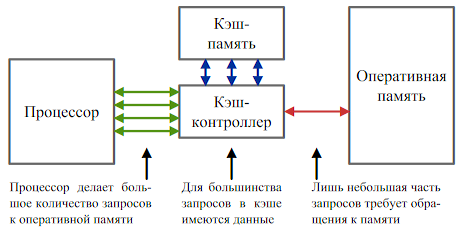
\includegraphics[scale=0.5]{fig1}}
		\caption{Общая схема кэш-памяти}
	\end{figure}
	
	Когда кэш перехватывает запросы к оперативной памяти, кэш-контроллер определяет, есть ли копия передаваемых данных в кэше. Если такая копия есть, то такая ситуация называется \textbf{кэш-попаданием} (hit), иначе - \textbf{кэш-промах} (miss). В случае, если кэш переполнен, работает политика замещения, которая определяет, какие данные должны быть вытеснены. Информация, хранящаяся в кэше, сопровождается метаинформацией (тэгом), который определяет, копией содержания какой ячейки является эта информация.
	
	Различают несколько уровней кэш-памяти процессора:\\
	- L1 Cache (кэш-память первого уровня) --- самая маленькая по объему, но самая быстрая и наиболее важная. Она содержит данные, наиболее часто используемые процессором и работает с минимальными задержками.\\
	- L2 Cache (кэш-память второго уроввня) --- по скорости уступает памяти L1, однако больше по объему. Она предназначена для временного хранения важной информации, вероятность обращения к которой ниже, чем у информации в кэше L1.\\
	- L3 Cache (кэш-память третьего уровня) --- самая большая по объему, но самая медленная, при этом скорость работы значительно выше скорости работы оперативной памяти. Она предназначена для хранения информации, вероятность обращения к которой ниже, чем у информации в L1 и L2. \cite{book:33862}\\
	\subsection{Отображение оперативной памяти на кэш-память}
	\subsubsection{Прямое отображение}
	
	Кэш-память прямого отображения является самой простой реализацией кэш-памяти. В кэш-памяти такого типа заданное слово может храниться только в одном месте. Если его в этом месте нет, то его нет в кэш-памяти вообще. Общая структура памяти с прямым отображением приведена на рисунке 2.
	\begin{figure}[h!]
		\center{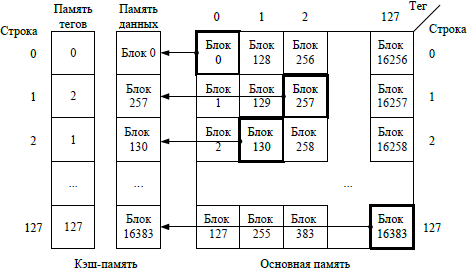
\includegraphics[scale=0.4]{fig2}}
		\caption{Схема памяти с прямым отображением}
	\end{figure}
	
	Как правило, формула отображения - есть остаток от деления адреса строки ОЗУ на количество строк кэш-памяти. При аппаратной реализации для получения адреса строки кэша достаточно убрать старшие биты адреса строки ОЗУ.\\
	Преимущества:\\
	- Простая реализация\\
	- Высокая скорость работы\\
	Недостатки:\\
	- Жесткое закрепление строк кэш-памяти за строками ОЗУ. Если будет обращение к разным блокам ОЗУ, которые отображаются на одни и те же строки кэш-памяти, это приведёт к снижению эффективности из-за постоянной перезаписи строк.
	\subsubsection{Полностью ассоциативное отображение}
	
	При полностью ассоциативном отображении любая ячейка ОЗУ может быть отображена на любую ячейку кэш-памяти. \\
	Преимущество:\\
	1. Возможность одновременно держать в кэш-памяти соседние ячейки ОЗУ.\\
	Недостатки:\\
	1. При большом количестве строк кэш-памяти задача нахождения нужной строки становится достаточно сложной с точки зрения аппаратной реализации.\\
	2. Более медленная, поскольку ассоциативная кэш-память работает последовательно.
	
	Схема полностью ассоциативного отображения приведена на рисунке 3. 
	
	\begin{figure}[h!]
		\center{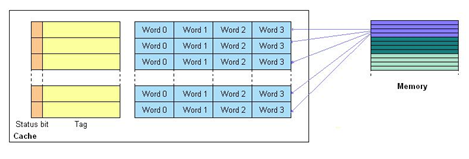
\includegraphics[scale=0.7]{fig3}}
		\caption{Схема памяти с полностью ассоциативным}
	\end{figure}
	\subsubsection{Множественно-ассоциативное отображением}\\
	    Компромиссом между предыдущими двумя методами является метод множественно-ассоциативного отображения. Кэш память разбивается на несколько подмножеств, называемых модулями. Блоки ОЗУ отображаются на модули также, как и при прямом отображении. Отображение строк внутри модуля является ассоциативном. Другими словами в каждом модуле могут присутствовать только строки из определенных блоков ОЗУ, а размещение строк внутри модуля является произвольным. В современных процессорах используется 4 и 8-канальная кэш-память. Увеличение числа ее входов приводит к быстрому увеличению сложности аппаратной реализации той части кэша, которая обеспечивает ассоциативный поиск тегов. Общая схема множественно-ассоциативного отображения приведена на рисунке 4.
	\begin{figure}[h!]
		\center{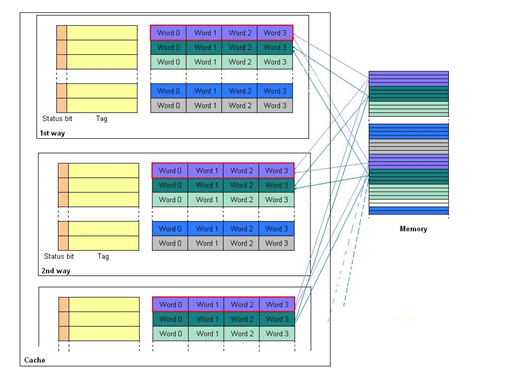
\includegraphics[scale=0.7]{fig4}}
		\caption{Схема памяти с множественно-ассоциативным отображением}
	\end{figure}
	\newpage
	\newpage
	\subsection{Замещение информации в кэш-памяти}
	\subsection{Запись в кэш-память}
	При возникновении промаха контроллер кэш-памяти должен выбрать подлежащую замещению строку. Для с прямого отображения аппаратные решения наиболее простые. На попадание проверяется только одна строка, и только эта строка может быть замещена. При полностью ассоциативной или множественно-ассоциативной организации кэш-памяти имеются несколько строк, из которых надо выбрать кандидата в случае промаха. Для решения этой задачи используют следующие специальные правила, называемые алгоритмами замещения.

1) FIFO (First In First Out – первый пришедший – первым выбывает);

2) LRU (Least Recently Used – дольше других неиспользуемый);

3) LFU (Least Frequently Used – реже других используемый);

4) Случайный (random).

Первый и последний методы являются самыми простыми в реализации, но они не учитывают, насколько часто используется та или иная строка КЭШ-памяти. При этом может быть удалена строка, к которой в самом ближайшем будущем будет обращение. Вероятность ошибки для указанных методов гораздо выше, чем у второго и третьего.

В алгоритме FIFO для замещения выбирается строка, первой попавшая в кэш. Каждая вновь размещаемая в кэше строка добавляется в конец этой очереди. Алгоритм не учитывает фактическое ее использование. Например, первые загруженные строки могут содержать данные, требующиеся на протяжении всей работы. Это приводит к немедленному возвращению к только что замещенной строке.

Алгоритм LRU предусматривает, что для удаления следует выбирать ту строку, которая не использовалась дольше других. При каждом обращении к строке ее временная метка обновляется. Это может быть сопряжено с существенными издержками. Однако алгоритм LRU наиболее часто используется на практике. Недостаток его заключается в том, что если программа проходит большой цикл, охватывающий множество строк, может случиться так, что строка, к которой дольше всего не было обращений, в действительности станет следующей используемой.

Одним из близких к LRU является алгоритм LFU, согласно которому удаляется наименее часто использовавшаяся строка. При этом необходимо подсчитывать количество обращений к каждой строке и контролировать его. Может оказаться, что наименее интенсивно используется та строка, которая только что записана в КЭШ-память и к которой успели обратиться только один раз (в то время как к другим строкам обращались больше). Она может быть удалена, что является недостатком алгоритма LFU.

Содержимое кэш-памяти меняется под управлением процессора. При этом основная память может оставаться неизменной. С другой стороны, внешние устройства могут изменять данные в ОП в режиме прямого доступа. При этом кэш-память не меняет своих данных. Еще сложнее ситуация в мультипроцессорных системах, когда несколько процессоров обращаются к общей памяти. Возникает проблема когерентности кэш-памяти.

Вычислительная система имеет когерентную память, если каждая операция чтения по адресу, выполненная каким-либо устройством, возвращает значение последней копии по этому адресу, независимо от того, какое из них производило запись последним. Проблема когерентности является наиболее важной для систем с обратным копированием. В них используются специальные протоколы, а к каждому тегу добавляются флаги модифицированности и достоверности информации. Эти флаги разрешают доступ к данным или запрещают его.
	\subsubsection{Прямая запись}
	\subsubsection{Обратная запись}
	\newpage
	\section{Реализация кэш-памяти}
	\subsection{Техническое задание}
	\textbf{Цель работы:} изучение основ структурного проектирования вычислительных систем, овладение современными САПР, получение навыков патентного поиска и исследовательской деятельности.\\
	
	1. Необходимо разработать систему памяти, включающую в себя кэш-память заданного размера. Система памяти должна принимать запросы на чтение/запись со стороны системной шины, выполнять поиск запрошенных данных в кэш-памяти. В случае кэш-промаха - перенаправлять запрос в контроллер оперативной памяти. Результаты запроса должны сохраняться в кэш, при необходимости вытеснив более старые данные в соответствии с заданным алгоритмом вытеснения. В случае кэш-попадания или после получения данных из ОП на запрос системной шины должен быть сформирован корректный ответ. Параметры системы памяти приведены в таблице 1.\\
	Системная шина, кэш память и интерфейс с ОП находятся в различных тактовых доменах.\\
	Интерфейс с \textbf{системной шиной} включает в себя следующие сигналы:
	
	\hspace{5mm}Входы: \textit{sys\_clk, sys\_rst\_n, sys\_addr[15:0], sys\_wr, sys\_rd, sys\_wdata[31:0], sys\_bval[31:0]}
	
	\hspace{5mm}Выходы: \textit{sys\_rdata[31:0], sys\_ack}\\
	Интерфейс с \textbf{контроллером оперативной памяти} включает в себя следующие сигналы:
	
	\hspace{5mm}Входы: \textit{ram\_clk, ram\_rst\_n, ram\_rdata[\textbf{31}:0], ram\_rack}
	
	\hspace{5mm}Выходы: \textit{ram\_addr[\textbf{11}:0], ram\_wdata[\textbf{31}:0], ram\_avalid, ram\_rnw}\\
	
	2. Провести патентный поиск по изобретениям и полезным моделям с глубиной поиска 25 лет (1994-2019) по заданным в таблице 1 алгоритмам и странам. Отчёт по поиску оформить в соответствии с ГОСТ Р 15.011-906, в т.ч. аналитическая часть. Таблица В.6.1, в приложении рефераты патентов.\\\\
	\begin{tabular}{ | p{200pt} | p{220pt} |}
	\hline
	Тип кэш-памяти & 8-ми канальная \\ \hline
	Объем кэш-памяти, байт & 2048 \\ \hline
    Разрядность шины данных ОП, байт & 4 \\ \hline
	Разрядность строки кэш-памяти, байт & 16 \\ \hline
	Алгоритм вытеснения & SLRU \\ \hline
	Алгоритм записи & прямая \\ \hline
	Алгоритмы для патентного поиска & записи \\ \hline
	Страны для патентного поиска & Россия, Франция, США \\ \hline
    \end{tabular}
    \begin{center}Таблица 1 --- Параметры задания (вариант 13)\end{center} \\\\
    Этапы выполнения работы:
    
    1. Подготовить обзор кэш-памяти;        
    
    2. Выполнить проектирование системы памяти;
    
    3. Провести патентный поиск;
    
    4. Подготовить пояснительную записку по выполненной работе.\\\\
    Базы данных для патентного поиска:\\\\
    \begin{tabular}{ | p{200pt} | p{220pt} |}
	\hline
	Роспатента & http://www.fips.ru \\ \hline
	ЕПВ Espacenet & http://ep.espacenet.com \\ \hline
    США USPATEULL & http://www.uspto.gov \\ \hline
	Google Patent Search & http://www.google.com/patent \\ \hline
	Всемирная организация интеллектуальной собственности (ВОИС) в системе PATENSCOPE & http://patentscope.wipo.int/search/en/search.jsf \\ \hline
    \end{tabular} 
    \newpage
	\subsection{Общее описание}
	
	В процессе проектирования системы памяти было сделано:
	
	1. Разработаны алгоритмы функционирования памяти тэгов, устройства управления, схемы замещения, алгоритмы чтения и записи в память;
	
	2. Разработана функциональная схема системы памяти и её компонентов согласно алгоритмам;
	
	3. Реализована система памяти на языке Verilog;
	
	4. Разработаны тесты компонентов, а также интеграционные тесты системы памяти на языке SystemVerilog.
	\subsection{Алгоритмы работы кэш-памяти}
	
	\subsection{Функциональная схема}
	\newpage
	\subsection{Описание модулей}
	\subsubsection{Память тэгов}
	Модуль памяти тегов отвечает за хранение тегов, а также обеспечивает вытеснение данных в случае, есть кэш-память заполнена. УГО модуля приведено на рисунке 5.\\
	\begin{figure}[h!]
		\center{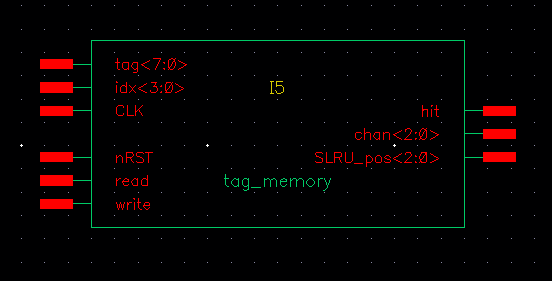
\includegraphics[scale=0.7]{fig5}}
		\caption{УГО памяти тегов}
	\end{figure}\\
	\textbf{Входы:}\\
	- CLK - вход синхронизации;\\
	- nRST - вход асинхронного сброса;\\
	- tag - тэг;\\
	- idx - индекс;\\
	- read - режим работы: чтение;\\
	- write - режим работы: запись.\\\\
	\textbf{Выходы:}\\
	- hit - сигнал, который устанавливается в 1 в случае кэш-попадания;\\
	- chan - номер канала, в котором обнаружено кэш-попадание.\\
	- SLRU\_pos - номер канала, из которого выталкивается очередная строка согласно схеме SLRU.
	
	\subsubsection{Память данных}
	Модуль памяти данных отвечает за хранение данных в секции, определяемой индексов и канале, который определяется памятью тегов.\\
	\begin{figure}[h!]
		\center{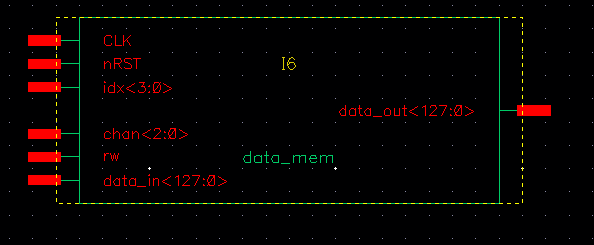
\includegraphics[scale=0.6]{fig6}}
		\caption{УГО памяти данных}
	\end{figure}\\\\
	\textbf{Входы:}\\
	- CLK - \\
	- nRST - \\
	- idx - \\
	- chan - \\
	- rw - \\
	- data\_in - \\
	\textbf{Выходы:}\\
	- data\_out - \\
	\subsubsection{Контроллер кэш-памяти}
	\begin{figure}[h!]
		\center{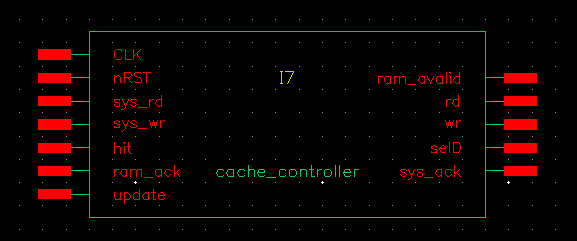
\includegraphics[scale=0.7]{fig7}}
		\caption{УГО кэш-контроллера}
	\end{figure}\\

    \begin{tikzpicture}[->, >=stealth', shorten >=1pt, auto, node    distance=4cm,thick, main node/.style={circle, draw, font=\sffamily\Large}]
    \node[initial right, state] (S1) {$S_1$};
    \node[state] (S2) [below=of S1] {$S_2$};
    \node[state] (S3) [left=of S1] {$S_3$};
    \node[state] (S4) [below left=of S3] {$S_4$};
    \node[state] (S5) [right=2cm of S4] {$S_5$};
    \node[state] (S6) [left= 2cm of S2] {$S_6$};
    
    \path[every node/.style={font=\sffamily\small}, label distance=9pt]
        (S1) edge [above] node[above=4pt] {$hit\And(sys\_rd\oplus sys\_wr)$} (S3)
        (S1) edge  node[sloped] {$ hit = 0$} (S2)
        (S2) edge  node[sloped] {$ram\_rack = 1$} (S6)
        (S6) edge  node {$ $} (S3)
        (S3) edge  node[above, sloped] {$Read$} (S4)
        (S3) edge  node[above, sloped] {$Write$} (S5)
        (S5) edge  node {$ $} (S4)
        (S4) edge  node {$ $} (S1); 
    \end{tikzpicture}

	\subsubsection{Модуль взаимодействия с ОЗУ}
	\begin{figure}[h!]
		\center{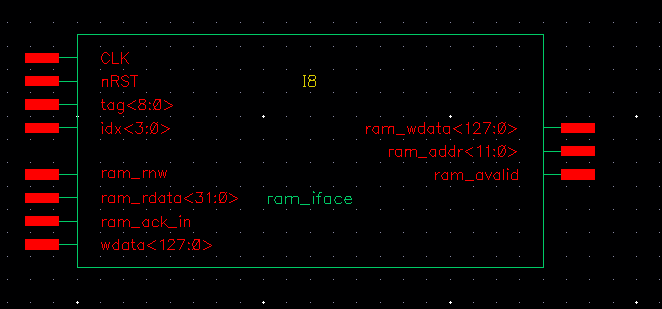
\includegraphics[scale=0.7]{fig8}}
		\caption{УГО модуля взаимодействия с ОЗУ}
	\end{figure}\\
	\subsubsection{Обработчик данных для записи}
	\begin{figure}[h!]
		\center{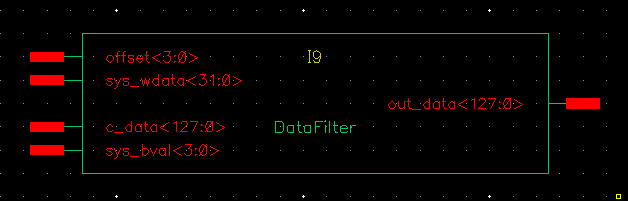
\includegraphics[scale=0.7]{fig9}}
		\caption{УГО обработчика данных}
	\end{figure}\\
	\begin{figure}[h!]
		\center{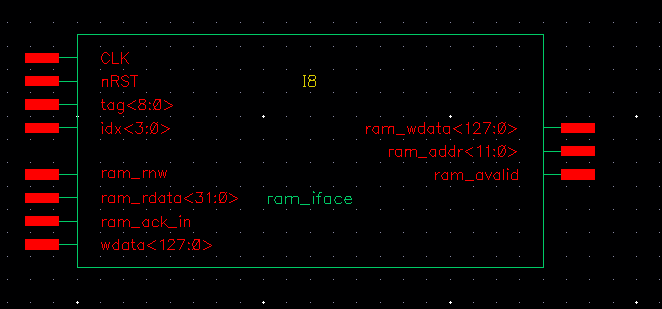
\includegraphics[scale=0.7]{fig8}}
		\caption{УГО модуля взаимодействия с ОЗУ}
	\end{figure}\\
	\newpage
	\section{Патентное исследование}
	\newpage
	\setcounter{secnumdepth}{-1}
	\section{Заключение}
	\newpage
	\printbibliography[heading=bibintoc]
	
\end{document}
